%\addcontentsline{toc}{chapter}{Development Process}
\chapter{Experiment Implementation}
\section{Summary}
To produce this research experiments must be run, and for this to happen experiments and the framework to carry them out need to be designed and implemented. This chapter will explain the key decisions and work carried out to produce our experimental results.

\section{Choice of Dataset}
For any machine learning task one of the first tasks that need to be undertaken once the nature of the task is determined is finding an appropriate dataset. The choice of dataset is important as it can dictate a number of our later decisions.

For image classification and labeling problems three of there are three common datasets that are used. We will briefly detail each one and choose which one to use.

There are of course other alternatives out there but these have been around for reasonably long and are small enough to work with the limited resources we had available at the start of the project.

\subsection{MNIST}
This dataset is a reduced subset of the NIST handwritten digit database and is made up of 60,000 hand written digits for training examples and 10,000 testing examples. The dimensions of each image is 28x28px.

These are used as a proof of concept for the neural network and a successful model using this dataset should be able to recognise a wide variety of normalised hand-written digits.

This dataset is considered one of the easiest of the ones we considered to perform well on, with top performing models getting accuracies as high as 99.79 percent.

\subsection{CIFAR-10}
This dataset was created using images harvested from the internet. It consists of 60,000 32x32 images organised into 10 classes hence its name. Each class is 6,000 images big and in addition contains 1,000 testing images per class for a total of 10,000 test images.

\begin{figure}
	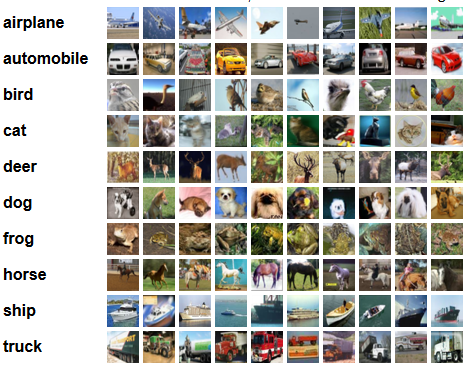
\includegraphics[width=0.8\linewidth]{cifar10}
	\caption{Example of CIFAR-10 images taken from CIFAR website}
\end{figure}

This figure shows some examples of the images that are available in the CIFAR-10 dataset in their respective classes. You will note that 'Truck' and 'Automobile' are both classes of image. However the dataset has been designed such that there is no intersection between classes so a 'Truck' cannot be an automobile and vice-versa.

\subsection{CIFAR-100}
The CIFAR-100 dataset is very similar to CIFAR-10. It contains the same number of images except we now have 100 classes of 600 training images and 20 superclasses for those 100 classes. Each class also includes 100 test images.

Both CIFAR-10 and 100 are created by the same group of people and are based on the same mined internet data.

Due to the lack of training examples and the significantly larger set of classes available, it is a much harder dataset to perform well in with top models getting 75.73 percent accuracy versus 96.53 percent for top performing CIFAR-10 results.

\subsection{The Verdict}
We ended up opting to focus our efforts on CIFAR-10. The reasoning was quite brief. MNIST is too simple and we tackled it early on for test runs. Results were reasonably high.

What we wished to present for our ending point in our project was a classifier which we wanted to use to classify internet images so MNIST wouldn't do for that.

CIFAR-100 on the other hand had features we were interested in trying to work with like the hierarchy which was interesting on the next project we want to do with this model but is quite difficult to get good results with and would push this projects beyond the scope of what can be done in MMP.

CIFAR-10 was a good compromise between the two so it was a good initial goal allowing us to scale to CIFAR-100 if we were satisfied with our results.

\section{Choice of Framework}
To start we need to decide how we are going to implement the neural networks. This involved several steps, of course one would be tempted to write their own implementation for an ANN, however that might be a major project on its own so a better solution is required.

We would like to minimise implementation effort in parts that do not improve the final project as much as possible so a library of some sort is necessary.

For our framework we wanted something that is both performant but also easy to use. We also want support for the latest ANN features while it needs to work on our workstation.

One of the greatest developments of the past 8 years in ANNs and machine learning in general is the advent and wide availability of parallel computing. Specifically GPU compute solutions like nVidia's CUDA technology have been invaluable in making Deep Neural Network research viable offering orders of magnitude better training times. Our frameword must run on a GPU.

We would like a library that makes testing an idea quickly, two modern candidates emerged at that point Google's new Tensor Flow software was one of them and was our favourite for the early parts of the project. Keras was another. Both use Python to define models and a backend implementation to do processing

We were not looking for specific features in this part of our project, what we were looking for however was a framework that is used in current research and is geared towards experimental CNNs both Keras and Tensor Flow support similar advanced CNN features which makes them fairly equivalent as a choice. They were both alpha software when the project started but so are most libraries in the field as CNNs are fairly new. We initially settled on Tensor Flow.

Most of the frameworks for this task are designed to work on Linux primarily. Tensor Flow works on Linux and OSX. This was a problem when we were running Windows on our main machine so the initial solution was to run Tensor Flow on a Virtual Machine with Linux Mint. This initially appeared to work well but we quickly discovered issues with this approach. To get good training performance CUDA is required. However CUDA requires a direct connection to the graphics adapter.

A solution we considered was to use Intel's VT-d and pass the PCI-E device of the GPU directly to the VM using the integrated Intel GPU in Windows instead allowing us to use it under a VM but this proved to be too complicated to set up and any other solution was equally complex. We had to abandon Tensor Flow. Keras, supported Windows as well so we ended up switching our efforts to that. This was relatively early on in the project's lifecycle so we could afford to make the change.

\section{The Stack}
\subsection{GPU Drivers and CUDA}
Because of the task of training and running through a neural network is an inherently parallel task we use Nvidia's CUDA technology in order to run computations on the GPU which produces at least an order of magnitude in performance gains over a modern traditional CPU architecture.

Nvidia's CUDA API has emerged as the dominant solution for scientific and industrial compute applications after competing open APIs like OpenCL failed to gain any traction. If you want good ANN performance CUDA is necessary.

\subsection{CuDNN}
CuDNN is an nVidia library written in C++ which provides performance optimisations for several ANN computations to run on CUDA enabled GPUs. This library isn't necessary, but it provided us with a significant performance boost so ended up being invaluable in our experiments.

\subsection{Backend Theano}
To execute computations we are using a library called Theano. Keras interacts with Theano and does weight computations on either the CPU or GPU giving a layer of compatibility and portability to our software as well as provides performance which is essential for training larger models. It uses CuDNN if it's installed to further increase performance on some nVidia GPUs.

\subsection{Keras}
Keras is a framework for creating and testing ANNs. This is the level our code directly interacts with. It provides us with implementations of ANN layers we use to build our models as well as data loaders analytics tools and more.

It can use either Theano or Tensor Flow as a backend to run its computations on the GPU or CPU. Theano then compiles the model in C++ which the CUDA SDK is compatible with.

\subsection{Our Application}
Inside our application we define models and hyper parameters which we are using to test. Our application trains a model and stops when a local minimum is identified for a set span of epochs and then saves the best model ie the local minimum. The model is then evaluated and a classification report is output.

There is methods also for loading models and to use a loaded model to classify an image input. These interfaces can be used to allow an external application to use our system.

\section {The Components of our Application}
Our code is organised in two major structures:
\subsection{Utilities}
This file contains implementations of some image processing algorithms as well as other utility functionality our program needs these are 'features' we use which aren't part of the experiment logic but enable certain experiments to be conducted.
\subsubsection{Colour Conversion}
A useful utility is the ability to convert training example between RGB colour and grayscale. We achieve this by implementing a number of conversion methods to try and extract the luminance of an RGB image. These methods range from averaging the intensity of the RGB channels at their simplest and least effective to weighted averages using the NTSC/W3C and Rec.702 colour weights for each RGB channel.

\subsubsection{Scaling and Cropping}
For this we use a library called OpenCV. Because our neural networks expect inputs to have certain dimensions we must first ensure that the pictures match. Aspect ration must first be matched by cropping trying to get the most prominent object in the cropped frame, then we scale to the desired size using OpenCV's scaling routines to match our ANN inputs.

\subsection{Main Program}
This comes in two separate forms, one is using a simple Multi-Layer Perceptron model and was used early in the project to obtain baseline results, the other is based on a Convolutional Neural Network model and was used in later development. The former was ported over to the framework used in the later for the final results. 

For all intents and purposes information applies to both unless otherwise noted.

\section{Challenges and Solutions}

\subsection{Data loading and pre-processing}
The first component of our training framework is loading of data. To do this we are taking advantage of built in Keras data loaders. For CIFAR-10/100 and MNIST these come packaged in and take care of downloading the data as well as loading it if it's not already provided. Tensor Flow and other frameworks also provide this.

After data is loaded we process it such that we extract information from it to determine the shape of the inputs and convert RGB values to a float32 value divided by 255. This gives us our ANN inputs. This is also where we do any splitting and colour conversion.

\subsubsection{Greyscale Luminance}
One of the main advantages and disadvantages of this process is it allows us to reduce the number of inputs into our ANN by a factor of 3. This in turn reduces training time by at least 50 percent which is a good advantage and greatly simplifies our network's structure. At the same time we reduce image detail which can have a negative impact in classification performance.

Because of the tradeoff we use both in our experiments, the faster training and simple models is appealing when trying a new hyper parameter for the first time and want to see quick results. Whereas higher performance is for when we have optimised all other aspects of the network.

We implemented our own colour conversion mechanisms that apply to a single image or sets of images. They are based on documentation for the NTSC and Rec.702 colourspaces as published in their respective standards. Exact references and discussion of the different sources for these are included in appendix 3.

\subsection{Regularisation}
As we explained in the previous chapter overfitting is a problem for ML and ANNs in particular, in a situation where we wish to achieve the best generalised performance. Training algorithms can only extract patterns from the data which they are given, so it follows that the more we train on data overfitting eventually takes place, i.e our classifier becomes more tailored to the training data at the expense of general performance.

Keras implements many ways to do this but what we are interested in is which ones we should use, in what variation where and how. How do they impact our performance metrics?

\subsubsection{Cross-Validation Split}
One of the most important problems to solve when combating overfitting is to be able to determine when it is happening so we may act on it.

What Keras enables us to do is to provide a set for validation which we can test against after each training epoch while we monitor our loss to train on our training data. Keras also has a feature to split a portion of the nth portion of the data for this purpose.

Our implementation is to use Keras's validation split for normal data and our own implementation for augmented data. This is because Keras until recently did not provide this feature for its data generator. In CIFAR-10 and 100 data is randomly distributed so we can just split the data at a point from the end and use that for this purpose.

What we do instead is we first shuffle in parallel the training data and labels then split the nth portion at the end. This approach would have been more useful if we were averaging runs. As it stands it means we have unnecessary variations in our data but our results were not visibly affected by this, we could have re-designed this omitting the shuffling or storing the seed for repeatability, but ideally we'd use Kera's better implementation instead now that it's available.

\subsubsection{Early Stopping and  Model Checkpoint}
Once we can monitor validation loss and can detect when a model might be overfitting we need something to act upon this. These methods are what we use.

Keras has a callback interface that allows us to call code in certain instances during training to do things. Early Stopping allows us to, with a patience parameter stop training when a model's validation results stop improving for a certain number of epochs. We use 50 epochs in most of our experiments. Because of how training works we want patience to be higher to avoid local minima since what we are looking for is actual local minimum validation loss.

Model checkpoint on the other hand solves another related issue. When validation results stop improving we stop after a few epochs but actually our best result might be several epochs old by the time we stop which means our model will already show signs of overfitting by the time it stops. We can avoid this issue by saving a copy of our most general model and loading it after our training has stopped and use that for validation.

\subsubsection{Data Augmentation}
Keras provides a capability to pass training data through a data generator before they are fed to the neural network for training. The idea is you can set filters that get applied randomly on each image such that every time you encounter an image in training it is slightly different in appearance.

The way this works is that by changing the actual pixel data in the inputs just enough so that the image features are intact you can mitigate the neural network overfitting to the data somewhat.

What we use is random rotation, which rotates the the image around its centrer by a random value of a given range, e.g. -1-1 degrees. Horizontal flip, which flips the image horizontally with a 50 percent likelyhood, and shifting the image by 2 pixels in either direction thus re-positioning it.

The filters work cyclically such that for n images n+1 image will be image 1 but each time the parameters of the filters will vary.

Another later consideration which came from a thought when we were examining data augmentation was to apply random noise to the inputs in hopes of reducing overfitting using the same principle. Keras does support the feature as a normalisation layer but at that point we already had data augmentation implemented and we found out that this kind of augmentation would be ill suited to the very small images we have in our network.

\subsubsection{Dropout}
We are using Keras implementation of dropout to reduce overfitting.

\subsection{Obtaining and visualising results}
For our experiments to be worth their salt we need to be able evaluate our models and visualise our results. For this we turn to SciKit Learn, which is an excellent library for machine learning statistics and visualisations. It helps us generate classification reports and confusion matrices which is the basis of our result reporting.

For evaluating the effects of our augmentations and our training and overfitting characteristics we are plotting loss and validation loss over time. This was a late addition to our framework so sadly we don't have much data for this.

We also initially intended to have a Google Inception-like visualisation of the learned features but we run out of time before implementing this.

\subsection{Saving Models}
Once a model is trained we save all our metrics with a label together with a serialised model and weights. This allows us to regenerate most reports as needed but also to use a trained model for whatever purposes we have.

\section{Our Basic Model}
We are basing our models on a standard Deep CNN architecture. This is very similar in appearance to something like figure \ref{CNNModel}

We are varying certain aspects of our model such that we can test the impact of changes in architectures and other hyper parameters in classification performance.

\begin{figure}
	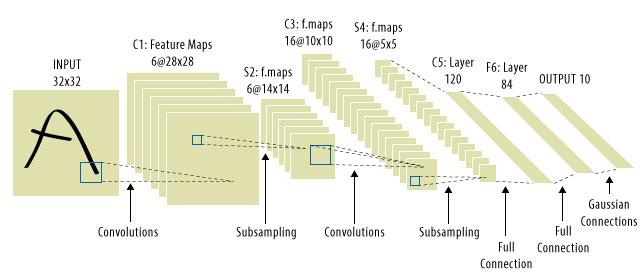
\includegraphics[width=0.8\linewidth]{common_cnn_design}
	\caption{Example of a common CNN design. See acknowledgements}
	\label{CNNModel}
\end{figure}